\documentclass[10pt,a4paper]{scrartcl}
\PassOptionsToPackage{table}{xcolor}
\usepackage[utf8]{inputenc}
\usepackage[T1]{fontenc}
\usepackage[ngerman]{babel}
\usepackage{microtype, multicol, marginnote, bera, parskip}
\usepackage{listings, amsmath, amssymb, graphicx, tikz, epic}
\usepackage{stmaryrd} %for lightning arrow
\usepackage{pstricks, pst-node, pst-tree, pdflscape}
\usepackage[babel=true]{csquotes}
\usepackage{placeins}
\usepackage[labelformat=empty]{caption}
\tolerance=2000
\setcounter{secnumdepth}{0}
\usepackage[inner=2cm,outer=2cm,top=1.5cm,bottom=1.5cm,includeheadfoot]{geometry}
\usepackage{multirow}
\usepackage{float}
\newcommand{\subExercise}[1]{\vspace{0.5em} \noindent{\bf #1)}}
\newcommand{\B}{\mathbb{B}}
\DeclareMathOperator{\op}{op}

\author{Michael Mardaus \and Andrey Tyukin}
\title{
\includegraphics[scale=0.2]{../logo_schriftzug}\\
Technische Informatik: Abgabe 10}

\begin{document}

\maketitle

\section*{Exercise 10.1 (7-Segment display PLA)}

Sorry, but I switched the order to most-significant-bit-first for the inputs.\\
So in order to be Question-compatible you have to exchange w and z; and x and y here.\\

Truthtable for LED-display\\
\begin{tabular}{|l||l|l|l|l||l|l|l|l|l|l|l|}\hline
i  & $w$ & $x$ & $y$ & $z$ &     $a$ & $b$ & $c$ & $d$ & $e$ & $f$ & $g$ \\\hline\hline
0  & 0   & 0   & 0   & 0   &      1  &  1  &  1  &  1  &  1  &  1  &  0  \\\hline
1  & 0   & 0   & 0   & 1   &      0  &  1  &  1  &  0  &  0  &  0  &  0  \\\hline
2  & 0   & 0   & 1   & 0   &      1  &  1  &  0  &  1  &  1  &  0  &  1  \\\hline
3  & 0   & 0   & 1   & 1   &      1  &  1  &  1  &  1  &  0  &  0  &  1  \\\hline
4  & 0   & 1   & 0   & 0   &      0  &  1  &  1  &  0  &  0  &  1  &  1  \\\hline
5  & 0   & 1   & 0   & 1   &      1  &  0  &  1  &  1  &  0  &  1  &  1  \\\hline
6  & 0   & 1   & 1   & 0   &      0  &  0  &  1  &  1  &  1  &  1  &  1  \\\hline
7  & 0   & 1   & 1   & 1   &      1  &  1  &  1  &  0  &  0  &  0  &  0  \\\hline
8  & 1   & 0   & 0   & 0   &      1  &  1  &  1  &  1  &  1  &  1  &  1  \\\hline
9  & 1   & 0   & 0   & 1   &      1  &  1  &  1  &  0  &  0  &  1  &  1  \\\hline
10 & 1   & 0   & 1   & 0   &      -  &  -  &  -  &  -  &  -  &  -  &  -  \\\hline
11 & 1   & 0   & 1   & 1   &      -  &  -  &  -  &  -  &  -  &  -  &  -  \\\hline
12 & 1   & 1   & 0   & 0   &      -  &  -  &  -  &  -  &  -  &  -  &  -  \\\hline
13 & 1   & 1   & 0   & 1   &      -  &  -  &  -  &  -  &  -  &  -  &  -  \\\hline
14 & 1   & 1   & 1   & 0   &      -  &  -  &  -  &  -  &  -  &  -  &  -  \\\hline
15 & 1   & 1   & 1   & 1   &      -  &  -  &  -  &  -  &  -  &  -  &  -  \\\hline
\end{tabular}

This leads to these K-maps:\\
\begin{tabular}{|c||c|c|c|c|}
  \hline
 $a$     & \multicolumn{4}{c|}{$yz$} \\
  $wx$   & 00                 & 01                 & 11                 & 10                 \\ \hline\hline
  00     & \cellcolor{gray}1  &                 0  & \cellcolor{gray}1  & \cellcolor{gray}1  \\ \hline
  01     &                 0  & \cellcolor{gray}1  & \cellcolor{gray}1  &                 0  \\ \hline
  11     & \cellcolor{gray}d  & \cellcolor{gray}d  & \cellcolor{gray}d  & \cellcolor{gray}d  \\ \hline
  10     & \cellcolor{gray}1  & \cellcolor{gray}1  & \cellcolor{gray}d  & \cellcolor{gray}d  \\ \hline
\end{tabular}
\begin{tabular}{|c||c|c|c|c|}
  \hline
 $b$     & \multicolumn{4}{c|}{$yz$} \\
  $wx$   & 00                 & 01                 & 11                 & 10                 \\ \hline\hline
  00     & \cellcolor{gray}1  & \cellcolor{gray}1  & \cellcolor{gray}1  & \cellcolor{gray}1  \\ \hline
  01     & \cellcolor{gray}1  &                 0  & \cellcolor{gray}1  &                 0  \\ \hline
  11     & \cellcolor{gray}d  &                 d  & \cellcolor{gray}d  &                 d  \\ \hline
  10     & \cellcolor{gray}1  & \cellcolor{gray}1  & \cellcolor{gray}d  & \cellcolor{gray}d  \\ \hline
\end{tabular}
\begin{tabular}{|c||c|c|c|c|}
  \hline
 $c$     & \multicolumn{4}{c|}{$yz$} \\
  $wx$   & 00                 & 01                 & 11                 & 10                 \\ \hline\hline
  00     & \cellcolor{gray}1  & \cellcolor{gray}1  & \cellcolor{gray}1  &                 0  \\ \hline
  01     & \cellcolor{gray}1  & \cellcolor{gray}1  & \cellcolor{gray}1  & \cellcolor{gray}1  \\ \hline
  11     & \cellcolor{gray}d  & \cellcolor{gray}d  & \cellcolor{gray}d  & \cellcolor{gray}d  \\ \hline
  10     & \cellcolor{gray}1  & \cellcolor{gray}1  & \cellcolor{gray}d  &                 d  \\ \hline
\end{tabular}
\begin{tabular}{|c||c|c|c|c|}
  \hline
 $d$     & \multicolumn{4}{c|}{$yz$} \\
  $wx$   & 00                 & 01                 & 11                 & 10                 \\ \hline\hline
  00     & \cellcolor{gray}1  &                 0  & \cellcolor{gray}1  & \cellcolor{gray}1  \\ \hline
  01     &                 0  & \cellcolor{gray}1  &                 0  & \cellcolor{gray}1  \\ \hline
  11     &                 d  & \cellcolor{gray}d  &                 d  & \cellcolor{gray}d  \\ \hline
  10     & \cellcolor{gray}1  &                 0  & \cellcolor{gray}d  & \cellcolor{gray}d  \\ \hline
\end{tabular}
\begin{tabular}{|c||c|c|c|c|}
  \hline
 $e$     & \multicolumn{4}{c|}{$yz$} \\
  $wx$   & 00                 & 01                 & 11                 & 10                 \\ \hline\hline
  00     & \cellcolor{gray}1  &                 0  &                 0  & \cellcolor{gray}1  \\ \hline
  01     &                 0  &                 0  &                 0  & \cellcolor{gray}1  \\ \hline
  11     &                 d  &                 d  &                 d  & \cellcolor{gray}d  \\ \hline
  10     & \cellcolor{gray}1  &                 0  &                 d  & \cellcolor{gray}d  \\ \hline
\end{tabular}
\begin{tabular}{|c||c|c|c|c|}
  \hline
 $f$     & \multicolumn{4}{c|}{$yz$} \\
  $wx$   & 00                 & 01                 & 11                 & 10                 \\ \hline\hline
  00     & \cellcolor{gray}1  &                 0  &                 0  &                 0  \\ \hline
  01     & \cellcolor{gray}1  & \cellcolor{gray}1  &                 0  & \cellcolor{gray}1  \\ \hline
  11     & \cellcolor{gray}d  & \cellcolor{gray}d  & \cellcolor{gray}d  & \cellcolor{gray}d  \\ \hline
  10     & \cellcolor{gray}1  & \cellcolor{gray}1  & \cellcolor{gray}d  & \cellcolor{gray}d  \\ \hline
\end{tabular}
\begin{tabular}{|c||c|c|c|c|}
  \hline
 $g$     & \multicolumn{4}{c|}{$yz$} \\
  $wx$   & 00                 & 01                 & 11                 & 10                 \\ \hline\hline
  00     &                 0  &                 0  & \cellcolor{gray}1  & \cellcolor{gray}1  \\ \hline
  01     & \cellcolor{gray}1  & \cellcolor{gray}1  &                 0  & \cellcolor{gray}1  \\ \hline
  11     & \cellcolor{gray}d  & \cellcolor{gray}d  & \cellcolor{gray}d  & \cellcolor{gray}d  \\ \hline
  10     & \cellcolor{gray}1  & \cellcolor{gray}1  & \cellcolor{gray}d  & \cellcolor{gray}d  \\ \hline
\end{tabular}

$a=w+xz+\bar x\bar z+yz$\\
$b=\bar x+\bar y\bar z+yz$\\
$c=\bar y+z+x$\\
$d=\bar x\bar z+x\bar yz+y\bar z+\bar xy$\\
$e=\bar x\bar z+y\bar z$\\
$f=w+\bar y\bar z+x\bar y+x\bar z$\\
$g=w+\bar xy+y\bar z+x\bar y$\\

This gives us this PLA:\\
\begin{tabular}{|c||c|c|c|c|c|c|c|c|c|c|c|c|c|c||c|}
  \hline
 input  & $w$ & $xz$ & $\bar x\bar z$ & $yz$ & $\bar y\bar z$ & $\bar x$ & $\bar y$ & $z$ & $x$ & $x\bar yz$ & $y\bar z$ & $\bar xy$ & $x\bar y$ & $x\bar z$ & output \\ \hline\hline
  $w$   & 2   & 0    &      0         &  0   &      0         &    0     &   0      &  0  &  0  &     0      &     0     &    0      &   0       &    0      &        \\ \hline
  $x$   & 0   & 2    &      3         &  0   &      0         &    3     &   0      &  0  &  2  &     2      &     0     &    3      &   2       &    2      &        \\ \hline
  $y$   & 0   & 0    &      0         &  2   &      3         &    0     &   3      &  0  &  0  &     3      &     2     &    2      &   3       &    0      &        \\ \hline
  $z$   & 0   & 2    &      3         &  2   &      3         &    0     &   0      &  2  &  0  &     2      &     3     &    0      &   0       &    3      &        \\ \hline\hline
        & 1   & 1    &      1         &  1   &      0         &    0     &   0      &  0  &  0  &     0      &     0     &    0      &   0       &    0      &   a    \\ \hline
        & 0   & 0    &      0         &  1   &      1         &    1     &   0      &  0  &  0  &     0      &     0     &    0      &   0       &    0      &   b    \\ \hline
        & 0   & 0    &      0         &  0   &      0         &    0     &   1      &  1  &  1  &     0      &     0     &    0      &   0       &    0      &   c    \\ \hline
        & 0   & 0    &      1         &  0   &      0         &    0     &   0      &  0  &  0  &     1      &     1     &    1      &   0       &    0      &   d    \\ \hline
        & 0   & 0    &      1         &  0   &      0         &    0     &   0      &  0  &  0  &     0      &     1     &    0      &   0       &    0      &   e    \\ \hline
        & 1   & 0    &      0         &  0   &      1         &    0     &   0      &  0  &  0  &     0      &     0     &    0      &   1       &    1      &   f    \\ \hline
        & 1   & 0    &      0         &  0   &      0         &    0     &   0      &  0  &  0  &     0      &     1     &    1      &   1       &    0      &   g    \\ \hline
\end{tabular}

We can optimize $x=x\bar z+xz$ so we could substitute the $x$ column above, so we would only need 13 columns. (I am sure there is more, but for the exercise it is \textit{optimized} now.)

\begin{tabular}{|c||c|c|c|c|c|c|c|c|c|c|c|c|c||c|}
  \hline
 input  & $w$ & $xz$ & $\bar x\bar z$ & $yz$ & $\bar y\bar z$ & $\bar x$ & $\bar y$ & $z$ & $x\bar yz$ & $y\bar z$ & $\bar xy$ & $x\bar y$ & $x\bar z$ & output \\ \hline\hline
  $w$   & 2   & 0    &      0         &  0   &      0         &    0     &   0      &  0  &     0      &     0     &    0      &   0       &    0      &        \\ \hline
  $x$   & 0   & 2    &      3         &  0   &      0         &    3     &   0      &  0  &     2      &     0     &    3      &   2       &    2      &        \\ \hline
  $y$   & 0   & 0    &      0         &  2   &      3         &    0     &   3      &  0  &     3      &     2     &    2      &   3       &    0      &        \\ \hline
  $z$   & 0   & 2    &      3         &  2   &      3         &    0     &   0      &  2  &     2      &     3     &    0      &   0       &    3      &        \\ \hline\hline
        & 1   & 1    &      1         &  1   &      0         &    0     &   0      &  0  &     0      &     0     &    0      &   0       &    0      &   a    \\ \hline
        & 0   & 0    &      0         &  1   &      1         &    1     &   0      &  0  &     0      &     0     &    0      &   0       &    0      &   b    \\ \hline
        & 0   & 1    &      0         &  0   &      0         &    0     &   1      &  1  &     0      &     0     &    0      &   0       &    1      &   c    \\ \hline
        & 0   & 0    &      1         &  0   &      0         &    0     &   0      &  0  &     1      &     1     &    1      &   0       &    0      &   d    \\ \hline
        & 0   & 0    &      1         &  0   &      0         &    0     &   0      &  0  &     0      &     1     &    0      &   0       &    0      &   e    \\ \hline
        & 1   & 0    &      0         &  0   &      1         &    0     &   0      &  0  &     0      &     0     &    0      &   1       &    1      &   f    \\ \hline
        & 1   & 0    &      0         &  0   &      0         &    0     &   0      &  0  &     0      &     1     &    1      &   1       &    0      &   g    \\ \hline
\end{tabular}

\FloatBarrier

\newpage
\section*{Exercise 10.2 (von-Neumann adder)}
We want to implement the computation unit of a von-Neumann adder by a PLA. 
The question is how many columns are required for addition of $n$-bit numbers.

\noindent{\textbf{Claim: }} The PLA has to have at least $3n$ columns.

\noindent{\textbf{Proof: }} 
We construct the Von-Neumann adder beginning on the end with the highest order bit carry,
and number the delays from left to right, as in the following figure:
\begin{figure}[H]
  \centering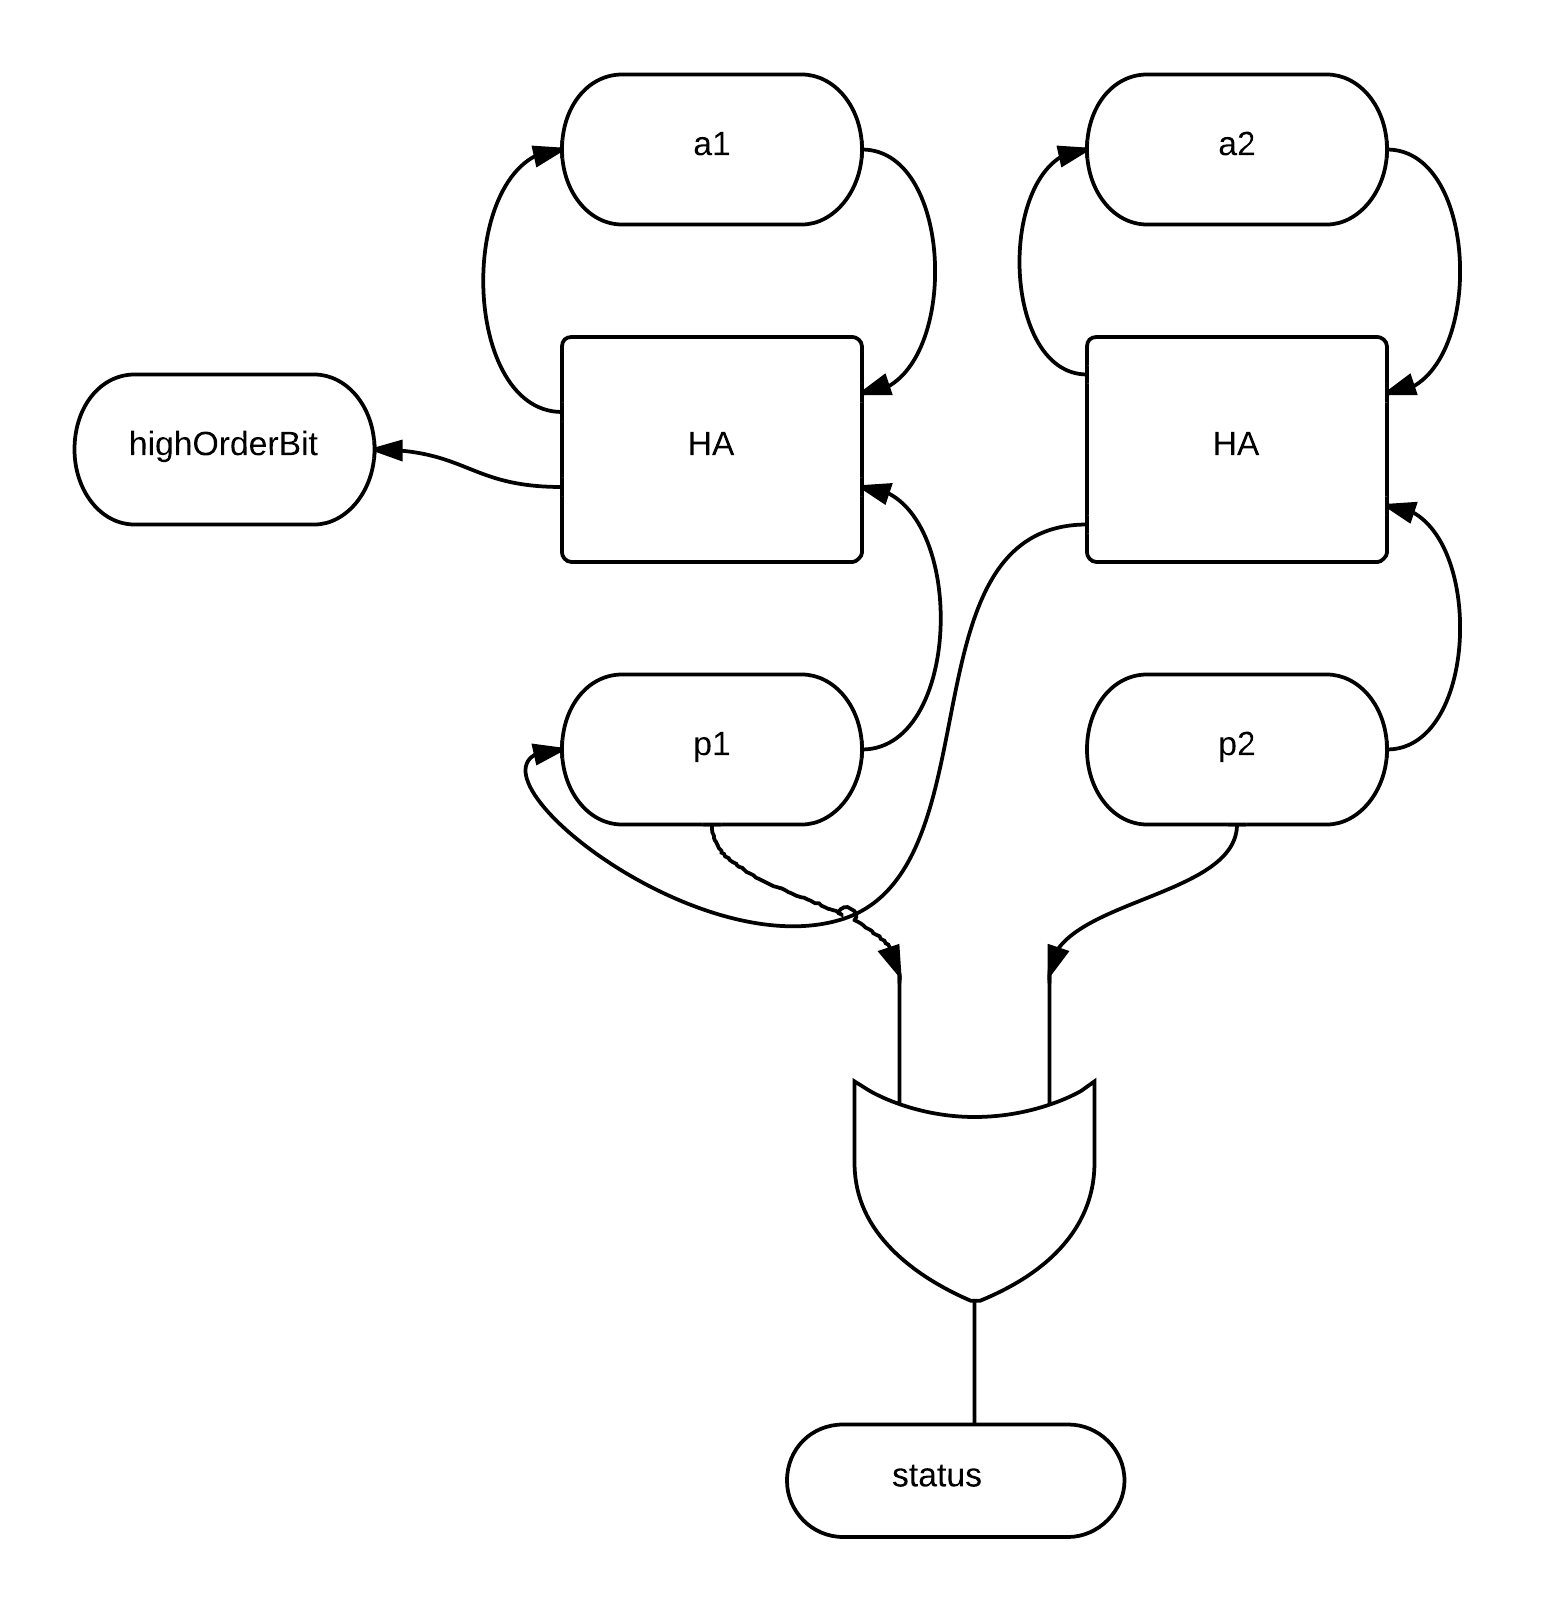
\includegraphics[width=0.6\linewidth]{images/vonNeumannAdder.png}
  \caption{Numbering of the registers for the von-Neumann adder is from left to right (CLK omitted)}
\end{figure}

Recall that the function we wish to implement is defined as follows:
\begin{align*}
  A_i &= a_i \bar p_i + \bar a_i p_i \\
  P_i &= \left\{\begin{array}{ll} a_{i+1}p_{i+1} & \textrm{ for } i<n \\ 0 \textrm{ for } i = n \end{array}\right. \\
  \mathrm{highOrderBit} &= a_1 p_1 \\
  \mathrm{status} &= \bigvee_{i=1}^{n-1} a_i p_i
\end{align*}

Thus, for each new digit we need three new minterms: $\bar a_i p_i, a_i\bar p_i, a_i p_i$.
Each of these minterms requires one new column in the PLA. 
The resulting PLA then looks as follows (most zeroes omitted):

\begin{figure}[H]
\centering\begin{tabular}{|c|ccc|ccc|ccc|ccc|c|}
  \hline
  $a_1$   &2&3&2& & & & & & & & & & \\
  $a_2$   & & & &2&3&2& & & & & & & \\
  $\vdots$& & & & & & &$\ddots$ &$\ddots$ &$\ddots$ & & & & \\
  $a_n$   & & & & & & & & & &2&3&2& \\
  \hline
  $p_1$   &2&2&3& & & & & & & & & & \\
  $p_2$   & & & &2&2&3& & & & & & & \\
  $\vdots$ & & & & & & &$\ddots$ &$\ddots$ &$\ddots$ & & & & \\
  $p_n$   & & & & & & & & & &2&2&3& \\
  \hline \hline
          &0&1&1& & & & & & & & & &$A_1$ \\
          & & & &0&1&1& & & & & & &$A_2$ \\
          & & & & & & &$\ddots$ &$\ddots$ &$\ddots$ & & & &$\vdots$\\
          & & & & & & & & & &0&1&1&$A_n$ \\
  \hline
          &1&0&0& & & & & & & & & & highOrderBit\\
  \hline
         & & & &1&0&0& & & & & & & $P_1$ \\
         & & & & & & &$\ddots$ &$\ddots$ &$\ddots$ & & & & $\vdots$ \\
         & & & & & & & & & &1&0&0& $P_{n-1}$ \\
         & & & & & & & & & & & & & $P_n$ \\
  \hline
         & & & &1&0&0&$\cdots$ & $\cdots$& $\cdots$&1 &0&0& status \\
  \hline

\end{tabular}
\end{figure}
Thus, the PLA consists of an AND part with $2n\times n$ blocks of size $1\times 3$ and an OR part with
$2n\times n$ blocks of size $1\times 3$. The total number of columns required is therefore $3n$.

\noindent{\textbf{Remark: }} 
As always, the dot-notation ($\cdots$) could be rewritten in a more formal inductive argument, 
but it is questionable whether it would make the explanation shorter or clearer. In this particular 
case, the dot-notation seemed much more readable.
\end{document}

